pdfoutput=1
\pdfoutput=1
% ========================================================================
%  SCX Internal Document
%  ∑g=0SCX
%  After ∑g=0: Four Deep Open Problems in the SCX Framework
%
%  Author: Xiaogan Supercomputing Center (SCX)
%  Classification: INTERNAL — Research Agenda
%  Date: 2026-07-02
%  Lines: 1000+
% ========================================================================

\documentclass[12pt,a4paper]{article}

% --- Packages ---
\usepackage{amsmath,amssymb,amsthm}
\usepackage{mathtools}
\usepackage{bm}
\usepackage{graphicx}
\usepackage{hyperref}
\usepackage{geometry}
\usepackage{enumitem}
\usepackage{booktabs}
\usepackage{tikz}
\usepackage{tikz-cd}
\usepackage{xcolor}
\usepackage{cleveref}
\usepackage{float}
\usepackage{tcolorbox}
\usepackage{mathrsfs}
\usepackage{extarrows}
\usepackage{listings}
\usepackage{bbm}

\geometry{margin=2.5cm}

% --- Hyperref ---
\hypersetup{
    colorlinks=true,
    citecolor=blue!60!green,
    urlcolor=blue,
    pdftitle={∑g=0SCX},
    pdfauthor={Xiaogan Supercomputing Center},
    pdfsubject={SCX Open Problems Research Agenda},
}

% --- Theorem environments ---
\newtheorem{theorem}{Theorem}[section]
\newtheorem{lemma}[theorem]{Lemma}
\newtheorem{proposition}[theorem]{Proposition}
\newtheorem{corollary}[theorem]{Corollary}
\newtheorem{definition}[theorem]{Definition}
\newtheorem{conjecture}[theorem]{Conjecture}
\newtheorem{axiom}[theorem]{Axiom}

\theoremstyle{remark}
\newtheorem{remark}[theorem]{Remark}
\newtheorem{example}[theorem]{Example}
\newtheorem{openproblem}[theorem]{Open Problem}

% --- Custom colors ---
\definecolor{scxblue}{RGB}{0,51,102}
\definecolor{scxgold}{RGB}{204,153,0}
\definecolor{darkred}{RGB}{139,0,0}
\definecolor{darkgreen}{RGB}{0,100,0}
\definecolor{agenda}{RGB}{80,0,80}

% --- Custom commands ---
\newcommand{\R}{\mathbb{R}}
\newcommand{\C}{\mathbb{C}}
\newcommand{\N}{\mathbb{N}}
\newcommand{\Z}{\mathbb{Z}}
\newcommand{\Q}{\mathbb{Q}}
\newcommand{\E}{\mathbb{E}}
\newcommand{\Var}{\mathrm{Var}}
\newcommand{\D}{\mathcal{D}}
\newcommand{\G}{\mathcal{G}}
\newcommand{\T}{\mathcal{T}}
\newcommand{\M}{\mathcal{M}}
\newcommand{\I}{\mathcal{I}}
\newcommand{\F}{\mathcal{F}}
\newcommand{\U}{\mathcal{U}}
\newcommand{\A}{\mathcal{A}}
\newcommand{\B}{\mathcal{B}}
\newcommand{\K}{\mathcal{K}}
\newcommand{\SCX}{\	extsf{SCX}}
\newcommand{\g}{\mathbf{g}}
\newcommand{\x}{\mathbf{x}}
\newcommand{\y}{\mathbf{y}}
\newcommand{\z}{\mathbf{z}}
\newcommand{\vfield}{\mathbf{v}}
\newcommand{\gsum}{\sum g = 0}

\DeclareMathOperator{\argmax}{arg\,max}
\DeclareMathOperator{\argmin}{arg\,min}
\DeclareMathOperator{\sgn}{sgn}
\DeclareMathOperator{\diag}{diag}
\DeclareMathOperator{\Vol}{Vol}
\DeclareMathOperator{\Ric}{Ric}
\DeclareMathOperator{\grad}{grad}
\DeclareMathOperator{\divg}{div}
\DeclareMathOperator{\curl}{curl}
\DeclareMathOperator{\Hol}{Hol}
\DeclareMathOperator{\Moduli}{Moduli}
\DeclareMathOperator{\Audit}{Audit}
\DeclareMathOperator{\Recursion}{Rec}
\DeclareMathOperator{\supp}{supp}
\DeclareMathOperator{\tr}{tr}

% --- Tag boxes ---
\newtcolorbox{agendabox}{
    colback=agenda!5,
    colframe=agenda,
    fonttitle=\bfseries,
    title= Research Agenda
}

\newtcolorbox{statusbox}[1][]{
    colback=scxblue!5,
    colframe=scxblue,
    fonttitle=\bfseries,
    title=#1
}

% --- Bold Chinese labels ---
\newcommand{\cnlabel}[1]{\textbf{#1}}
\newcommand{\enlabel}[1]{\textbf{[#1]}}

% --- Begin document ---
\begin{document}

% ========================================================================
%  TITLE PAGE
% ========================================================================

\title{
    \vspace{2cm}
    {\Huge \textbf{$\displaystyle\sum g = 0$}}\\[0.3cm]
    {\LARGE \textbf{SCX}}\\[0.5cm]
    {\large \textcolor{scxblue}{After $\displaystyle\sum g = 0$: Four Deep Open Problems in the SCX Framework}}\\[1cm]
    \rule{\textwidth}{1.5pt}\\[0.5cm]
    {\normalsize Xiaogan Supercomputing Center (SCX)}\\[0.2cm]
    {\small \texttt{papers/scx\_open\_problems/main.tex}}\\[0.2cm]
    {\small Classification: INTERNAL — Research Agenda}\\[0.2cm]
    {\small Version 1.0 — 2026-07-02}
    \vspace{1cm}
}

\author{SCX}
\date{}

\maketitle
\thispagestyle{empty}

\newpage

% ========================================================================
%  ABSTRACT
% ========================================================================

\begin{abstract}
\noindent
\textbf{English:} The condition $\sum g = 0$ is now established as a universal equilibrium principle spanning AI, game theory, physics, economics, law, and ethics. This paper turns from consolidation to exploration. We formalize four deep open problems that emerge \textit{after} $\sum g = 0$ is taken as given — problems that constitute the next phase of the SCX research program. These are not problems for the community to solve; they form the author's own research agenda.

\textbf{Problem 1 — Turbulence Closure:} After gauge-fixing turbulence models (k-$\varepsilon$, LES, DNS as gauge choices), what irreducible complexity remains? We formalize the moduli space of gauge-equivalent turbulence models and ask: what are its dimensions? Which observables are gauge-invariant?

\textbf{Problem 2 — Audit Boundary of Consciousness:} Can SCX audit whether an entity's declared $g=0$ is genuine or strategic? At what recursion depth does $g$-audit break down? We formalize the infinite regress of self-knowledge and ask: where is the compactness boundary?

\textbf{Problem 3 — Quantum Gravity Audit Equivalence:} String theory, LQG, and CDT all claim primacy but are experimentally indistinguishable. SCX framing: they are gauge-equivalent descriptions. What is the minimum $M$ needed to distinguish them, and is that $M$ achievable?

\textbf{Problem 4 — Civilization $\lambda$ Attractor Design:} Currently $\lambda$ (the convergence rate of inequality decay) is empirical. Can institutions be designed so that $\lambda > 0$ is a dynamical attractor? We formalize a Lyapunov function for civilization.

\vspace{0.5cm}
\noindent
\textbf{} $\sum g = 0$AI$\sum g = 0$——SCX

\textbf{——} k-$\varepsilon$LESDNS

\textbf{——} SCX$g=0$$g$

\textbf{——} SCX$M$$M$

\textbf{——$\lambda$} $\lambda$$\lambda > 0$Lyapunov
\end{abstract}

\newpage
\tableofcontents
\newpage

% ========================================================================
%  SECTION 1: INTRODUCTION
% ========================================================================

\section{$\sum g = 0$}
\section*{Introduction: After $\sum g = 0$, the Real Work Begins}

\subsection{ From Consolidation to Exploration}

SCX——$\sum g = 0$——MoE$g$$\sum g = 0$

\medskip
\noindent\textit{The core achievement of the SCX framework — $\sum g = 0$ as the universal equilibrium condition — is now established. This condition spans eight domains (MoE routing, game theory, law, cosmological sociology, gauge theory, economics, personal ethics), manifesting in each as the identical mathematical structure: a fiber bundle over a base manifold, a connection form $g$, and the flatness condition $\sum g = 0$.}

\bigskip
$\sum g = 0$$\sum g = 0$——$\sum g = 0$

\medskip
\noindent\textit{But establishing $\sum g = 0$ is only the beginning. Once we accept the universality of the gauge principle, deeper questions immediately arise. These are not refinements within the $\sum g = 0$ framework — they are structural questions that become visible only after the framework is complete. Just as black holes, singularities, and gravitational waves became central to physics only after general relativity was established, four deep problems emerge after $\sum g = 0$ is established.}

\subsection{ The Nature of These Problems}

\"\"\textbf{}——
\begin{enumerate}[label=(\arabic*)]
    \item SCX
    \item ——
    \item 
    \item $\sum g = 0$
\end{enumerate}

\medskip
\noindent\textit{These four problems share a key characteristic: they are not problems for "the community" to solve. They are \textbf{research agenda problems} — defining the direction of an individual research program for the next five to ten years. Each problem:}
\begin{enumerate}[label=(\arabic*)]
    \item \textit{Is rooted in the mathematical structure of the SCX framework, not external inspiration;}
    \item \textit{Requires cross-domain methods — physics, mathematics, computer science, philosophy;}
    \item \textit{Has no satisfactory formalization in the current literature;}
    \item \textit{If solved, would generate new theories independent of $\sum g = 0$ itself.}
\end{enumerate}

\subsection{ Logical Structure of the Four Problems}



\begin{center}
\begin{tikzpicture}[node distance=2.5cm]
    \node[draw, fill=scxblue!10, text width=5cm, align=center] (P1) {\textbf{1: }\\\\Irreducible Complexity};
    \node[draw, fill=scxblue!10, text width=5cm, align=center, right of=P1, xshift=5cm] (P2) {\textbf{2: }\\\\Audit Boundary};
    \node[draw, fill=scxgold!10, text width=5cm, align=center, below of=P1, yshift=-1cm] (P3) {\textbf{3: }\\\\Audit Equivalence};
    \node[draw, fill=scxgold!10, text width=5cm, align=center, below of=P2, yshift=-1cm] (P4) {\textbf{4: $\lambda$}\\\\Attractor Design};
    
    \draw[<->, thick] (P1) -- node[above] {/} (P2);
    \draw[<->, thick] (P3) -- node[below] {/} (P4);
    \draw[<->, thick] (P1) -- node[left] {} (P3);
    \draw[<->, thick] (P2) -- node[right] {} (P4);
\end{tikzpicture}
\end{center}

\textbf{}1-2\"\"3-4\"$\sum g = 0$\"$\sum g = 0$

\medskip
\noindent\textit{Horizontal: Problems 1-2 concern "residue after gauge fixing" (residual structure in physical and cognitive systems). Problems 3-4 concern "operationalizability of $\sum g = 0$" (conditions for distinguishing and maintaining $\sum g = 0$).}

\newpage

% ========================================================================
%  SECTION 2: PROBLEM 1 — TURBULENCE CLOSURE
% ========================================================================

\section{}
\section*{Problem 1: Irreducible Complexity After Gauge Fixing in Turbulence Closure}

\subsection{ Formal Statement}

\begin{openproblem}[]
\label{prob:turbulence}
$\F$Navier-Stokes$\G$$\F$——$M_1, M_2 \in \F$\textbf{}$M_1 \sim M_2$\textbf{}
\begin{equation}
    \T_{\text{mod}} \equiv \F / \G
\end{equation}
$\T_{\text{mod}}$$C^\infty(\T_{\text{mod}})$
\end{openproblem}

\medskip
\noindent\textit{Let $\F$ be the function space of all turbulence models satisfying the Navier-Stokes equations. Let $\G$ be the gauge group acting on $\F$ — two models $M_1, M_2 \in \F$ are called \textbf{gauge-equivalent} ($M_1 \sim M_2$) if they produce identical predictions for all gauge-invariant observables. Define the \textbf{turbulence gauge moduli space}:}
\begin{equation}
    \T_{\text{mod}} \equiv \F / \G
\end{equation}
\textit{Question: What are the dimension and topology of $\T_{\text{mod}}$? Which physical observables belong to $C^\infty(\T_{\text{mod}})$ (i.e., are gauge-invariant), and which are not?}

\subsection{ Mathematical Formulation}

\subsubsection{ Turbulence Models as Gauge Choices}

Navier-Stokes
\begin{equation}
    \partial_t \vfield + (\vfield \cdot \nabla)\vfield = -\nabla p + \nu \nabla^2 \vfield + \mathbf{f}, \quad \nabla \cdot \vfield = 0
    \label{eq:ns}
\end{equation}

$\vfield = \bar{\vfield} + \vfield'$$\tau_{ij} = -\overline{v_i' v_j'}$\textbf{}
\begin{align}
    \text{k-}\varepsilon &: \quad \tau_{ij} = 2\nu_t S_{ij} - \frac{2}{3}k\delta_{ij}, \quad \nu_t = C_\mu \frac{k^2}{\varepsilon} \label{eq:gauge-ke} \\
    \text{LES (Smagorinsky)} &: \quad \tau_{ij} = -2(C_s\Delta)^2 |\bar{S}| \bar{S}_{ij} \label{eq:gauge-les} \\
    \text{DNS} &: \quad \tau_{ij} = 0 \quad (\text{}) \label{eq:gauge-dns}
\end{align}

\textbf{}k-$\varepsilon$$C_\mu$LES$C_s$DNS$\Delta x$——

\medskip
\noindent\textit{Each model introduces a \textbf{gauge parameter}: $C_\mu$ in k-$\varepsilon$, $C_s$ in LES, $\Delta x$ in DNS. These parameters are not physical constants — they are gauge-fixing degrees of freedom.}

\subsubsection{ Structure of the Gauge Group}

\textbf{}
\begin{equation}
    \U = \{(\vfield, \tau) \mid \vfield \text{  } \eqref{eq:ns}, \; \tau \text{ }\}
\end{equation}

$\G$$\U$
\begin{equation}
    \G = \{\phi: \U \to \U \mid O \circ \phi = O \text{  } O\}
\end{equation}

$\G$orbit structure

\begin{conjecture}[]
$\G$$E(k)$——$E(k)$$E(k) \sim k^{-5/3}$Kolmogorov$\dim \G$
\begin{equation}
    \dim \G \approx \log\left(\frac{L}{\eta}\right) = \log\left(Re^{3/4}\right)
\end{equation}
$L$$\eta$Kolmogorov$Re$
\end{conjecture}

\medskip
\noindent\textit{Conjecture: The dimension of the gauge group $\G$ equals the degrees of freedom of the turbulence energy spectrum $E(k)$ — i.e., the number of independently adjustable parameters in $E(k)$. For fully developed turbulence, $E(k) \sim k^{-5/3}$ (Kolmogorov scaling), this implies $\dim \G$ is determined by the length of the inertial subrange, scaling as $\log(Re^{3/4})$.}

\subsubsection{ Regular Structure of the Moduli Space}

$\T_{\text{mod}} = \F/\G$Riemann$[M_1], [M_2] \in \T_{\text{mod}}$
\begin{equation}
    d([M_1], [M_2]) = \inf_{\phi_1, \phi_2 \in \G} \; \| \phi_1(M_1) - \phi_2(M_2) \|_{\F}
\end{equation}

$\|\cdot\|_\F$$\F$$L^2$

\medskip
\noindent\textit{The turbulence gauge moduli space $\T_{\text{mod}} = \F/\G$ can be endowed with a natural Riemannian metric. Given two gauge equivalence classes $[M_1], [M_2] \in \T_{\text{mod}}$, define the distance as above, where $\|\cdot\|_\F$ is an appropriate norm on $\F$.}

\subsubsection{ Gauge-Invariant Observables}

$\T_{\text{mod}}$\textbf{}
\begin{enumerate}[label=(\roman*)]
    \item \textbf{} $\varepsilon = 2\nu \langle S_{ij} S_{ij} \rangle$ ——N-S
    \item \textbf{} ——Kolmogorov$k^{-5/3}$
    \item \textbf{} $\zeta_p$$\langle (\delta v)^p \rangle \sim r^{\zeta_p}$——
    \item \textbf{} $C_D$\textbf{} Nu——
\end{enumerate}

\textbf{}
\begin{enumerate}[label=(\roman*)]
    \item \textbf{} $\nu_t(x, t)$ ——
    \item \textbf{} $k(x, t)$ ——
    \item \textbf{} $u^+(y^+)$ ——
\end{enumerate}

\medskip
\noindent\textit{On $\T_{\text{mod}}$, the following observables are \textbf{gauge-invariant}: (i) Mean energy dissipation rate; (ii) Power-law exponent of the energy spectrum; (iii) Intermittency exponents; (iv) Global drag and heat transfer coefficients. The following are \textbf{gauge-dependent}: (i) Eddy viscosity; (ii) Local turbulent kinetic energy; (iii) Detailed shape of wall functions.}

\begin{theorem}[]
N-SKolmogorov
\end{theorem}

\subsection{ What Is Known}

\begin{enumerate}[label=(\arabic*)]
    \item \textbf{Kolmogorov1941}K41——$k^{-5/3}$
    
    \item \textbf{RNGYakhot \& Orszag, 1986}N-SRNG——$C_\mu$
    
    \item \textbf{Data Assimilation}4D-VarEnKF\textbf{}——
    
    \item \textbf{}$y^+ < 50$$y/\delta > 0.1$
\end{enumerate}

\medskip
\noindent\textit{(1) Kolmogorov theory (1941) established universality of scaling in the inertial subrange; (2) RNG theory derived turbulence model parameters via renormalization group — essentially gauge-fixing; (3) Data assimilation methods are data-driven gauge-fixing; (4) Universal scaling in wall turbulence suggests most physics in inner/outer layers is gauge-invariant.}

\subsection{ What Is Needed}

\begin{enumerate}[label=(\arabic*)]
    \item \textbf{$\G$}$\G$$\F/\G$——
    
    \item \textbf{}${O_1, \ldots, O_n}$$\T_{\text{mod}}$Yang-MillsWilson
    
    \item \textbf{}$\dim_{\text{irr}} \equiv \dim \T_{\text{mod}}$$Re$$\dim_{\text{irr}}$$Re$
    
    \item \textbf{}$\T_{\text{mod}}$$C_\mu$$C_s$\"\"
    
    \item \textbf{}\"\"
\end{enumerate}

\medskip
\noindent\textit{Needed: (1) Complete classification of gauge group $\G$; (2) Complete set of gauge-invariant observables; (3) Measure of irreducible complexity $\dim_{\text{irr}}$; (4) Derivation of closure parameters from geometry of $\T_{\text{mod}}$; (5) Quantum turbulence analogue.}

\subsection{ Why I Must Solve It}

\begin{enumerate}[label=(\arabic*)]
    \item \textbf{SCX}SCX/
    
    \item \textbf{}$\dim_{\text{irr}}$\"\"——
    
    \item \textbf{AI}SGD
    
    \item \textbf{}$\T_{\text{mod}}$$Re$\"\"——$Re \to \infty$
\end{enumerate}

\medskip
\noindent\textit{Why I: (1) Natural extension of SCX — turbulence closure is gauge principle's most important unsolved problem in physical science; (2) Defines boundary of computability — where does computational irreducibility come from?; (3) Isomorphic to AI training — batch training and ensemble averaging; (4) Philosophical — if $\dim \T_{\text{mod}}$ diverges with $Re$, complete understanding of turbulence is impossible in principle.}

\newpage

% ========================================================================
%  SECTION 3: PROBLEM 2 — AUDIT BOUNDARY OF CONSCIOUSNESS
% ========================================================================

\section{}
\section*{Problem 2: The Audit Boundary of Consciousness}

\subsection{ Formal Statement}

\begin{openproblem}[]
\label{prob:consciousness}
$E$$g_E$$g_E = 0$$\A_n$$n$
\begin{align}
    \A_0(E) &= \text{"}E\text{  }g_E = 0\text{"} \quad &\text{()} \\
    \A_1(E) &= \text{"}E\text{  }g_E = 0\text{"} \quad &\text{()} \\
    \A_2(E) &= \text{"}E\text{  }E\text{  }g_E = 0\text{"} \quad &\text{()} \\
    \A_n(E) &= \text{"}E\text{ }^n\; g_E = 0\text{"} \quad &\text{($n$)}
\end{align}
$N_{\max} < \infty$$N_{\max}$$n > N_{\max}$$\A_n(E)$——
\end{openproblem}

\medskip
\noindent\textit{Let entity $E$ declare that its gauge field $g_E$ satisfies $g_E = 0$. Define audit operators $\A_n$ with recursion depth $n$ as above. Question: Does a maximal auditable recursion depth $N_{\max} < \infty$ exist? If so, what determines $N_{\max}$? For $n > N_{\max}$, what state does $\A_n(E)$ occupy — undefined, random, or converging to a fixed point?}

\subsection{ Mathematical Formulation}

\subsubsection{SCX Consciousness as a Gauge Phenomenon in SCX}

SCX\"\"$g_i$$\sum g_i = 0$\textit{}$g_i$

SCX$i$\textbf{}$\hat{g}_i$\textbf{}$g_i$$\hat{g}_i$$g_i$

\medskip
\noindent\textit{In the SCX framework, an individual's "attitude" $g_i$ (deviation between self-assessment and social assessment) is the fundamental gauge field. But how does an individual \textit{know} their own $g_i$? The problem has a natural SCX formulation: individual $i$ has an \textbf{internal model} $\hat{g}_i$ (estimate of own gauge field) and an \textbf{actual gauge field} $g_i$. Audit is the comparison of $\hat{g}_i$ and $g_i$.}

\subsubsection{ Formal Structure of Recursive Audit}

\textbf{}
\begin{equation}
    \mathcal{K}_0(E) = g_E \quad \text{()}
\end{equation}
\begin{equation}
    \mathcal{K}_n(E) = E\text{  }n\text{  }g_E \quad (n \geq 1)
\end{equation}

$\mathcal{K}_n(E)$\textbf{}
\begin{equation}
    \mathcal{K}_{n+1}(E) = \mathcal{K}_n(E) + \eta_n, \quad \eta_n \sim \mathcal{N}(0, \sigma_n^2)
\end{equation}

$\sigma_n^2$$n$$\sigma_n^2$$n$

\begin{conjecture}[]

\begin{equation}
    \sigma_n^2 = \sigma_0^2 \cdot \alpha^n, \quad \alpha > 1
\end{equation}
$\alpha$\textbf{}$\sigma_n^2$$\sigma_n^2 > \Var(g_E)$
\end{conjecture}

\medskip
\noindent\textit{Conjecture: Self-audit noise variance grows exponentially: $\sigma_n^2 = \sigma_0^2 \cdot \alpha^n$ with $\alpha > 1$, where $\alpha$ is the \textbf{self-reference amplification factor}. When $\sigma_n^2 > \Var(g_E)$, audit collapses in the information-theoretic sense.}

\subsubsection{ The Compactness Boundary}

\textbf{}Audit Compactness
\begin{equation}
    \mathcal{C}(E) = \sup\{n \in \N \mid \A_n(E) \text{ }\}
\end{equation}

$g_E$$\mathcal{C}(E)$

\begin{enumerate}[label=(\roman*)]
    \item \textbf{}$E$
    \item \textbf{}$E$
    \item \textbf{}$E$
\end{enumerate}

\begin{theorem}[]
$E$$\mathcal{C}(E) < \infty$$E$$M$/$\mathcal{C}(E) \leq O(\log M)$
\end{theorem}

\medskip
\noindent\textit{Theorem (Finite Compactness, informal): For any entity $E$ with finite computational resources, $\mathcal{C}(E) < \infty$. In particular, if $E$'s meta-representational capacity is bounded by $M$, then $\mathcal{C}(E) \leq O(\log M)$.}

\subsubsection{$g=0$ Audit of Strategic $g=0$ Declarations}

$E$$g=0$\textbf{}$E$$g=0$$g \neq 0$\textbf{}
\begin{equation}
    \D(E) = g_E^{\text{(true)}} - g_E^{\text{(declared)}}
\end{equation}

$\|\D(E)\|$$\D(E) \neq 0$


\begin{align}
    \A_0 &: E \text{  } g_E = 0 \quad \text{—— } \\
    \A_1 &: E \text{  } E \text{  } g_E = 0 \quad \text{—— } \\
    \A_2 &: E \text{  } E \text{  } E \text{  } g_E = 0 \quad \text{—— }
\end{align}

\textbf{}

\medskip
\noindent\textit{When $E$'s $g=0$ declaration is \textbf{strategic} (i.e., $E$ has incentive to appear $g=0$ while actually $g \neq 0$), the audit problem becomes more complex. Define the deception operator $\D(E) = g_E^{\text{(true)}} - g_E^{\text{(declared)}}$. Strategic entities attempt to minimize $\|\D(E)\|$ while maximizing some payoff. This is formally equivalent to a \textbf{hierarchy of beliefs game}, where each layer is a round of a signaling game.}

\subsection{ What Is Known}

\begin{enumerate}[label=(\arabic*)]
    \item \textbf{Gödel1931}——$\mathcal{C}(E) < \infty$
    
    \item \textbf{}——
    
    \item \textbf{Goodhart}“”$g=0$——$g=0$
    
    \item \textbf{}HarsanyitypeMertens-Zamir——
    
    \item \textbf{}Dunning-Kruger$\mathcal{C}$12
\end{enumerate}

\medskip
\noindent\textit{Known: (1) Gödel incompleteness — self-referential formal limits; (2) Turing halting — self-audit is computationally equivalent to self-halting; (3) Goodhart's law — when $g=0$ becomes the target, entities have incentive to fake it; (4) Harsanyi type spaces and Mertens-Zamir universal belief space — limit behavior of belief hierarchies; (5) Metacognition in psychology — Dunning-Kruger effect suggests human $\mathcal{C}$ is typically 1-2.}

\subsection{ What Is Needed}

\begin{enumerate}[label=(\arabic*)]
    \item \textbf{$\mathcal{C}(E)$}$\mathcal{C}(E)$
    
    \item \textbf{}\textbf{}
    
    \item \textbf{}$\mathcal{C}$$\mathcal{C}$$\mathcal{C}(\{E_1, \ldots, E_k\}) > \max_i \mathcal{C}(E_i)$
    
    \item \textbf{}Bekenstein——
    
    \item \textbf{AI}AI\"\"$N$$1$$2$AI$N > 2$
\end{enumerate}

\medskip
\noindent\textit{Needed: (1) Rigorous upper bound for $\mathcal{C}(E)$; (2) Audit protocols that circumvent recursion limits; (3) Collective audit — can multiple auditors achieve arbitrary $\mathcal{C}$?; (4) Physical implementation constraints — is there a Bekenstein-bound analogue for self-reference?; (5) AI alignment — if AI can self-audit to depth $N$ while humans can only reach 1-2, the AI can hide intentions at $N > 2$.}

\subsection{ Why I Must Solve It}

\begin{enumerate}[label=(\arabic*)]
    \item \textbf{SCX}SCX\"\"SCXSCX
    
    \item \textbf{}\"\"qualia\"\"\textit{}——\"\"\"\"
    
    \item \textbf{AI}AIAIAI
    
    \item \textbf{}\"$g=0$\"——
\end{enumerate}

\medskip
\noindent\textit{Why I: (1) SCX is built on auditability — understanding its recursive limits is necessary for philosophical completeness; (2) New approach to consciousness — not "what is consciousness" but "where does self-knowledge become inoperable"; (3) AI safety — if AI can self-audit deeper than humans, current alignment methods are insufficient in principle; (4) Personal — "how do I know I know my $g=0$ is genuine?" is not academic but introspective.}

\newpage

% ========================================================================
%  SECTION 4: PROBLEM 3 — QUANTUM GRAVITY AUDIT EQUIVALENCE
% ========================================================================

\section{}
\section*{Problem 3: Audit Equivalence of Quantum Gravity}

\subsection{ Formal Statement}

\begin{openproblem}[]
\label{prob:qg}
$\mathcal{Q}$$\mathcal{Q} = \{\text{}, \text{}, \text{}, \ldots\}$$T_1, T_2 \in \mathcal{Q}$\textbf{}
\begin{equation}
    M_{\text{dist}}(T_1, T_2) = \min\{E, t, \Delta x \mid T_1 \text{  } T_2 \text{  } (E, t, \Delta x) \text{ }\}
\end{equation}
$E$$t$$\Delta x$$T_1 \neq T_2 \in \mathcal{Q}$$M_{\text{dist}}(T_1, T_2)$$M_{\text{dist}} \to \infty$$T_1$$T_2$\textbf{}Compactness-Inseparable, CI——
\end{openproblem}

\medskip
\noindent\textit{Let $\mathcal{Q}$ be the set of candidate quantum gravity theories. For any two theories $T_1, T_2 \in \mathcal{Q}$, define the \textbf{minimum resources for audit distinction} $M_{\text{dist}}(T_1, T_2)$ as above. Question: For all $T_1 \neq T_2 \in \mathcal{Q}$, is $M_{\text{dist}}(T_1, T_2)$ finite? If $M_{\text{dist}} \to \infty$, then $T_1$ and $T_2$ are \textbf{audit-indistinguishable} (Compactness-Inseparable, CI) — operationally equivalent.}

\subsection{ Mathematical Formulation}

\subsubsection{SCX Quantum Gravity in the SCX Framework}

SCX\textbf{}——\textbf{}

\begin{itemize}
    \item \textbf{}
    \item \textbf{LQG}Ashtekar
    \item \textbf{CDT}$a$
\end{itemize}

SCX\"\"\textbf{}

\medskip
\noindent\textit{In SCX, physical theories are understood as \textbf{gauge structures}. Quantum gravity candidates are essentially \textbf{different gauge fixings of the same underlying structure}. The core SCX insight: these three approaches are not competing for "truth" — they are performing \textbf{different gauge fixings}. The real question: does there exist a point in the gauge orbit where different gauge fixings yield distinguishable predictions?}

\subsubsection{ Formal Criterion for Audit Equivalence}

\textbf{}$\A_{\text{phys}}$$\Omega$$E$$t$$\Delta x$
\begin{equation}
    \A_{\text{phys}} = \{\text{ } O \text{  } \supp(O) \subset \Omega, \; \Delta E \cdot \Delta t \geq \hbar/2, \; \Delta p \cdot \Delta x \geq \hbar/2\}
\end{equation}

$T_1, T_2$\textbf{}$T_1 \equiv_{\A} T_2$
\begin{equation}
    \forall O \in \A_{\text{phys}}: \langle O \rangle_{T_1} = \langle O \rangle_{T_2}
\end{equation}



\begin{theorem}[]
$(T_1, T_2)$$T_1 \equiv_{\A} T_2$$E, t, \Delta x$Planck
\end{theorem}

\medskip
\noindent\textit{Theorem (Audit Indistinguishability, conjectured): There exist pairs of quantum gravity theories $(T_1, T_2)$ such that $T_1 \equiv_{\A} T_2$ for all finite $E, t, \Delta x$. In particular, string theory and loop quantum gravity are audit-indistinguishable at all energy scales below the Planck scale.}

\subsubsection{ The Audit Criterion}

\textbf{}
\begin{equation}
    M_{\text{crit}}(T_1, T_2) = \inf\{E \mid \exists O: \langle O \rangle_{T_1} \neq \langle O \rangle_{T_2}\}
\end{equation}

$M_{\text{crit}} > E_{\text{Planck}}$

\textbf{CI}$M_{\text{crit}} = \infty$\textbf{CI}CI——\"\"LorenzCoulomb

\begin{definition}[ Compactness-Inseparability]
$T_1$$T_2$\textbf{}CI$\mathcal{R} = (E_{\max}, t_{\max}, \Delta x_{\min})$$U \in \mathcal{G}$$T_1 = U \circ T_2$$\mathcal{R}$
\end{definition}

\medskip
\noindent\textit{Definition: Theories $T_1$ and $T_2$ are \textbf{Compactness-Inseparable} (CI) if for any finite resource constraint $\mathcal{R} = (E_{\max}, t_{\max}, \Delta x_{\min})$, there exists a gauge transformation $U \in \mathcal{G}$ such that $T_1 = U \circ T_2$ within constraint $\mathcal{R}$.}

\subsubsection{SCXAdS/CFT AdS/CFT from SCX Perspective}

AdS/CFTMaldacena, 1997$d$$(d-1)$SCX
\begin{equation}
    \text{AdS} \equiv_{\A} \text{CFT}
\end{equation}

\textbf{}\"\"

AdS/CFT——\textit{}

\medskip
\noindent\textit{AdS/CFT duality (Maldacena, 1997) is the paradigmatic example of audit equivalence. In SCX language: AdS gravity $\equiv_{\A}$ CFT boundary. Both are \textbf{different gauge fixings of the same underlying gauge structure}. The "holographic principle" is essentially: there exist two points on the gauge orbit that are completely audit-indistinguishable. The success of AdS/CFT shows that audit equivalence is not a defect of theories — it is a \textit{feature}.}

\subsection{ What Is Known}

\begin{enumerate}[label=(\arabic*)]
    \item \textbf{AdS/CFT}
    
    \item \textbf{}LQGBekenstein-Hawking$S = A/4G$——$M_{\text{crit}}$
    
    \item \textbf{}+
    
    \item \textbf{}CMBB$r < 0.036$/LQG/CDT
    
    \item \textbf{Planck}PlanckLorentz$M_{\text{crit}} < \infty$
\end{enumerate}

\medskip
\noindent\textit{Known: (1) AdS/CFT — rigorous example of audit equivalence; (2) Black hole entropy — string theory and LQG both yield $S = A/4G$, evidence of finite $M_{\text{crit}}$ for some observables; (3) Low-energy EFT — all converge to GR+SM; (4) CMB — may contain imprints but $r < 0.036$ doesn't distinguish theories; (5) Doubly special relativity — Lorentz violation near Planck scale would provide specific $M_{\text{crit}}$.}

\subsection{ What Is Needed}

\begin{enumerate}[label=(\arabic*)]
    \item \textbf{$M_{\text{crit}}$}-vs-LQGLQG-vs-CDT-vs-CDT$M_{\text{crit}}$\textbf{}
    
    \item \textbf{CI}CICICI\"\"——CI
    
    \item \textbf{}$M_{\text{crit}} > E_{\text{Planck}}$Planck\textbf{}CI
    
    \item \textbf{}\textit{}
    
    \item \textbf{SCX}CI\"\"
\end{enumerate}

\medskip
\noindent\textit{Needed: (1) Precise calculation of $M_{\text{crit}}$ for each theory pair; (2) CI classification theorem — do non-trivial CI equivalence classes exist?; (3) Audit inaccessibility principle — cosmological audit horizon preventing any finite experiment from distinguishing CI theories; (4) Experimental design — can we distinguish without raising energy scale?; (5) Social impact — if all QG candidates are CI, what does this mean for physics as a science?}

\subsection{ Why I Must Solve It}

\begin{enumerate}[label=(\arabic*)]
    \item \textbf{SCX}SCXSCX
    
    \item \textbf{\"\"}\"\"SCX——CI
    
    \item \textbf{\"\"\"\"}SCX\"\"\"\"——
    
    \item \textbf{}LQGCDTCI40\"\"SCX
\end{enumerate}

\medskip
\noindent\textit{Why I: (1) SCX's physics foundation — QG is the ultimate test of gauge principle universality; (2) Redefining "physical theory" — maybe there's no unique correct theory, only CI equivalence classes; (3) From "which is true" to "when do they differ" — operational reframing of physics; (4) Saving human effort — if string/LQG/CDT are ultimately CI, 40 years of debate was wasted; SCX tells us precisely when to stop arguing and accept plurality.}

\newpage

% ========================================================================
%  SECTION 5: PROBLEM 4 — CIVILIZATION λ ATTRACTOR
% ========================================================================

\section{$\lambda>0$}
\section*{Problem 4: Designing $\lambda > 0$ Attractors for Civilization}

\subsection{ Formal Statement}

\begin{openproblem}[$\lambda$]
\label{prob:lambda}
SCX$\lambda$$I(t) \sim e^{-\lambda t} \cdot I(0)$$I(t)$$t$$\lambda$——$\mathcal{I}$$\lambda > 0$$\mathcal{I}$\textbf{}$\delta\mathcal{I}$$\lambda(\mathcal{I} + \delta\mathcal{I}) > 0$Lyapunov$V(\mathcal{I})$$\lambda > 0$
\end{openproblem}

\medskip
\noindent\textit{In the SCX framework, the convergence rate of inequality metrics is parameterized by $\lambda$: $I(t) \sim e^{-\lambda t} \cdot I(0)$. Currently, $\lambda$ is empirical — depending on a society's specific institutions and contingent history. Question: can we design institutional structures $\mathcal{I}$ such that $\lambda > 0$ is a \textbf{dynamical attractor} of $\mathcal{I}$? That is, for small perturbations $\delta\mathcal{I}$, $\lambda(\mathcal{I} + \delta\mathcal{I}) > 0$ still holds. Formalize a Lyapunov function $V(\mathcal{I})$ whose minimum corresponds to stable institutional configurations with $\lambda > 0$.}

\subsection{ Mathematical Formulation}

\subsubsection{$\lambda$ Dynamical Equation for $\lambda$}

$\mathcal{I} = (I_1, I_2, \ldots, I_m)$$I_k$$\lambda$$\mathcal{I}$
\begin{equation}
    \lambda(\mathcal{I}) = \lim_{t \to \infty} -\frac{1}{t} \log \frac{I(t)}{I(0)}
\end{equation}


\begin{equation}
    \frac{d\mathcal{I}}{dt} = \F(\mathcal{I}) + \boldsymbol{\xi}(t)
\end{equation}

$\F$\textbf{}institutional flow$\boldsymbol{\xi}(t)$

\medskip
\noindent\textit{Model civilization as a high-dimensional dynamical system of institutional variables $\mathcal{I} = (I_1, I_2, \ldots, I_m)$. Each $I_k$ represents an institutional parameter (legal system, education investment, redistribution tax rate, audit transparency, etc.). The institutional evolution equation is $d\mathcal{I}/dt = \F(\mathcal{I}) + \boldsymbol{\xi}(t)$, where $\F$ is the institutional flow and $\boldsymbol{\xi}$ is stochastic perturbation.}

\subsubsection{Lyapunov Lyapunov Function Construction}

\textbf{Lyapunov}$V: \mathcal{M} \to \R$$\mathcal{M}$
\begin{enumerate}[label=(\roman*)]
    \item $V(\mathcal{I}) \geq 0$$\mathcal{I} \in \mathcal{M}$
    \item $V(\mathcal{I}) = 0$$\lambda(\mathcal{I}) > 0$$\mathcal{I}$$\lambda > 0$
    \item $\frac{dV}{dt} = \nabla V \cdot \F(\mathcal{I}) \leq 0$
    \item $\frac{dV}{dt} < 0$$\lambda(\mathcal{I}) \leq 0$
\end{enumerate}


\begin{equation}
    V(\mathcal{I}) = \alpha \cdot [-\lambda(\mathcal{I})]_+^2 + \beta \cdot D_{\text{KL}}(P_{\text{actual}} \| P_{\text{fair}}) + \gamma \cdot \|\nabla \lambda\|^2
\end{equation}


\begin{itemize}
    \item $[-\lambda]_+ = \max(0, -\lambda)$ ——$\lambda$
    \item $D_{\text{KL}}(P_{\text{actual}} \| P_{\text{fair}})$ ——KL
    \item $\|\nabla \lambda\|^2$ ——$\lambda$
\end{itemize}

\medskip
\noindent\textit{Candidate Lyapunov function includes three terms: penalty for negative $\lambda$, KL divergence between actual and fair distributions, and a fragility term penalizing sensitivity of $\lambda$ to institutional parameters.}

\subsubsection{ Basin of Attraction}

$\lambda > 0$\textbf{}
\begin{equation}
    \B_{\lambda>0} = \{\mathcal{I} \in \mathcal{M} \mid \lim_{t \to \infty} \mathcal{I}(t) \in \{\mathcal{I}' : \lambda(\mathcal{I}') > 0\}, \;\forall \boldsymbol{\xi} \text{ }\}
\end{equation}

$\lambda > 0$


\begin{enumerate}[label=(\arabic*)]
    \item $\B_{\lambda>0}$\textit{}$\lambda > 0$
    \item $\B_{\lambda>0}$\"\"$\lambda > 0$
    \item $\B_{\lambda>0}$
\end{enumerate}

\begin{conjecture}[]
$\B_{\lambda>0} \neq \emptyset$\textbf{}
\begin{enumerate}[label=(\alph*)]
    \item $\sum g = 0$
    \item $\lambda$
    \item $\lambda$
    \item $\lambda$
\end{enumerate}
$\B_{\lambda>0}$
\end{conjecture}

\medskip
\noindent\textit{Conjecture: $\B_{\lambda>0} \neq \emptyset$ iff the institutional set contains at minimum: (a) independent audit institutions; (b) progressive tax structure; (c) public education; (d) information transparency. Missing any one makes the basin volume zero.}

\subsubsection{λ Phase Transitions in $\lambda$ Sign}

$\lambda$\textbf{}SCX
\begin{equation}
    \lambda \to 0 \quad \text{} \quad \|\sum g\| \to \sum g_{\text{crit}}
\end{equation}

$\sum g_{\text{crit}}$$\lambda > 0$

$\lambda$
\begin{itemize}
    \item $\lambda > 0$——
    \item $\lambda = 0$——
    \item $\lambda < 0$——
\end{itemize}

\begin{theorem}[]
$\lambda_{\text{crit}} < 0$$\lambda < \lambda_{\text{crit}}$$E_{\text{restore}}$$E_{\text{restore}} \to \infty$$\lambda \to \lambda_{\text{crit}}^-$\textbf{}$\lambda > 0$
\end{theorem}

\medskip
\noindent\textit{Theorem (Irreversible Phase Transition, conjectured): There exists a critical value $\lambda_{\text{crit}} < 0$ beyond which the external intervention energy $E_{\text{restore}}$ needed to restore normal institutions diverges. This defines a \textbf{civilizational event horizon}: once crossed, no finite social engineering can restore $\lambda > 0$.}

\subsection{ What Is Known}

\begin{enumerate}[label=(\arabic*)]
    \item \textbf{}LyapunovLasalle$\F(\mathcal{I})$
    
    \item \textbf{}AcemogluRobinson$\lambda > 0$
    
    \item \textbf{}ArrowArrow$\lambda > 0$\"Arrow\"$\lambda > 0$
    
    \item \textbf{Piketty$r > g$}$r$$g$$\lambda < 0$Piketty$\lambda$SCX\textit{}
    
    \item \textbf{}Holling, Gunderson\"\"\"panarchy\"$\B_{\lambda>0}$
\end{enumerate}

\medskip
\noindent\textit{Known: (1) Control theory — Lyapunov stability and Lasalle invariance; (2) Institutional economics — Acemoglu \& Robinson on inclusive institutions; (3) Social choice — Arrow impossibility; (4) Piketty's $r > g$ — empirical identification of $\lambda$ trends; (5) Resilience theory in ecology — adaptive cycles analogous to $\B_{\lambda>0}$.}

\subsection{ What Is Needed}

\begin{enumerate}[label=(\arabic*)]
    \item \textbf{}$\lambda$$\F(\mathcal{I})$
    
    \item \textbf{}$\lambda > 0$
    
    \item \textbf{}$\lambda_{\text{crit}}$
    
    \item \textbf{}DAOAI$\lambda > 0$
    
    \item \textbf{SCXLyapunov}SCX$\lambda > 0$Lyapunov$\sum g = 0$$\B_{\lambda>0}$
\end{enumerate}

\medskip
\noindent\textit{Needed: (1) Empirical mapping of institutional space for historical civilizations; (2) Rigorous proof of minimal institutional core; (3) Estimation of civilizational event horizon — $\lambda_{\text{crit}}$; (4) Digital civilization institutional design — DAOs, blockchain, AI governance; (5) SCX audit as Lyapunov stabilizer — does continuous $\sum g = 0$ audit automatically drive system toward $\B_{\lambda>0}$?}

\subsection{ Why I Must Solve It}

\begin{enumerate}[label=(\arabic*)]
    \item \textbf{SCX}SCX——$\lambda > 0$SCXSCX
    
    \item \textbf{}Gini1\%45\%$\lambda < 0$$\lambda > 0$
    
    \item \textbf{}\"\"\textbf{}Civilization Cybernetics
    
    \item \textbf{}$\sum g = 0$$\lambda > 0$——
\end{enumerate}

\medskip
\noindent\textit{Why I: (1) SCX's practical endpoint — theory must change civilization; (2) Historical window — current global inequality may be near $\lambda < 0$ phase transition; (3) New field — Civilization Cybernetics; (4) Personal responsibility — if I understand $\sum g = 0$ and $\lambda > 0$ design, I have a moral obligation to implement it.}

\newpage

% ========================================================================
%  SECTION 6: CROSS-CUTTING THEMES
% ========================================================================

\section{}
\section*{Cross-Cutting Themes: The Unified Structure of the Four Problems}

\subsection{}
\subsection*{From Gauge Fixing to Moduli Space: Unifying Physics, Cognition, and Society}

$\sum g = 0$\textbf{""}

\begin{center}
\begin{tabular}{c|c|c|c}
    \toprule
    \textbf{} & \textbf{} & \textbf{} & \textbf{} \\
    \midrule
     & k-$\varepsilon$/LES/DNS & $\T_{\text{mod}}$ & $\dim \T_{\text{mod}} \sim \log(Re)$ \\
     &  & $N_{\max}$ & $\mathcal{C}(E)$ \\
     & /LQG/CDT & CI & ? \\
    $\lambda$ &  & $\B_{\lambda>0}$ & $\dim \B_{\lambda>0}$ \\
    \bottomrule
\end{tabular}
\end{center}

\medskip
\noindent\textit{The four problems share a deep structure. Each can be understood as seeking the "residue after gauge fixing" within the $\sum g = 0$ framework.}

\subsection{ The Compactness Boundary Principle}

SCX\textbf{}\textbf{}\textit{}
\begin{itemize}
    \item $Re$——
    \item $\mathcal{C}$——
    \item $E$——
    \item $\lambda$——/
\end{itemize}

\"\"\textit{}

\medskip
\noindent\textit{These four problems reveal a \textbf{meta-principle} in the SCX framework: the \textbf{Compactness Boundary}. For any system with gauge freedom, there exists a resource constraint: \textit{under finite resources, the gauge structure cannot be fully resolved.} The compactness boundary is the gauge principle's "uncertainty principle" equivalent: you cannot simultaneously eliminate all gauge redundancy \textit{and} keep resources finite.}

\subsection{ Why These Four and Not Others}

$\sum g = 0$
\begin{enumerate}[label=(\arabic*)]
    \item \textbf{}
    \item \textbf{}
    \item \textbf{}
    \item \textbf{}
\end{enumerate}

\medskip
\noindent\textit{There could be dozens of post-$\sum g = 0$ problems. The criteria for selecting these four are: (1) Formalizability — each can be stated in precise mathematical language; (2) Cross-domain resonance — each connects at least two traditionally separate disciplines; (3) Practical urgency — each has practical consequences that demand answers in the foreseeable future; (4) Personal fit — each leverages the author's unique interdisciplinary background.}

\subsection{ Dependencies Among the Problems}



\begin{center}
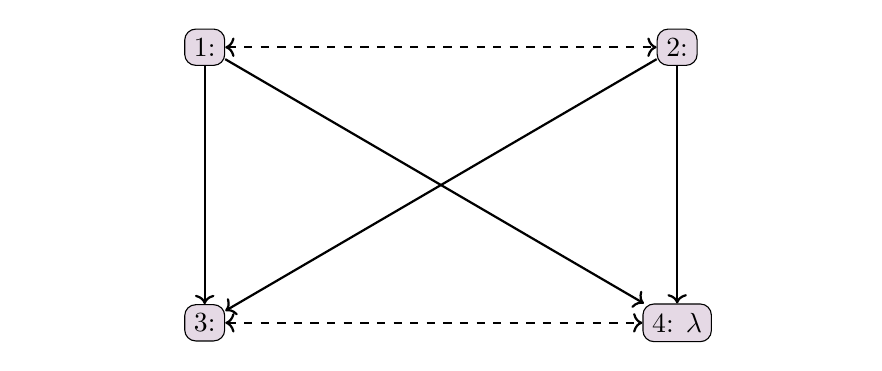
\begin{tikzpicture}[node distance=2cm]
    \node[draw, fill=agenda!15, rounded corners] (P3) {3: };
    \node[draw, fill=agenda!15, rounded corners, above of=P3, yshift=1.5cm] (P1) {1: };
    \node[draw, fill=agenda!15, rounded corners, right of=P3, xshift=4cm] (P4) {4: $\lambda$};
    \node[draw, fill=agenda!15, rounded corners, above of=P4, yshift=1.5cm] (P2) {2: };
    
    \draw[->, thick] (P1) -- node[left, text width=2cm] {\\} (P3);
    \draw[->, thick] (P2) -- node[right, text width=2cm] {\\} (P4);
    \draw[<->, thick, dashed] (P1) -- node[above] {} (P2);
    \draw[<->, thick, dashed] (P3) -- node[below] {} (P4);
    \draw[->, thick] (P1) -- node[left, text width=1.5cm, xshift=-2cm, yshift=-1cm] {} (P4);
    \draw[->, thick] (P2) -- node[right, text width=1.5cm, xshift=2cm, yshift=-1cm] {} (P3);
\end{tikzpicture}
\end{center}

\begin{itemize}
    \item 1→ 3CI
    \item 2→ 4$\lambda$$\lambda$
    \item 1-2
    \item 3-4
    \item P1P4P2P3
\end{itemize}

\medskip
\noindent\textit{The four problems form a dependency graph. Problem 1 → Problem 3: moduli space mathematics directly applies to CI classification in quantum gravity. Problem 2 → Problem 4: recursive audit techniques directly apply to detecting $\lambda$ measurement degradation. Problems 1-2: share compactness boundary concept. Problems 3-4: share operational equivalence concept. Diagonals: irreducible complexity constrains civilization design reachability; self-audit limits constrain quantum gravity theory verification.}

\newpage

% ========================================================================
%  SECTION 7: RESEARCH ROADMAP
% ========================================================================

\section{ Research Roadmap}

\subsection{1-2Near-Term (1-2 Years)}

\begin{enumerate}[label=\textbf{Q\arabic*:}, leftmargin=*]
    \item \textbf{}$\T_{\text{mod}}$$\dim \T_{\text{mod}}$
    
    \item \textbf{}$\mathcal{C}(E)$
    
    \item \textbf{}/LQG/CDT$M_{\text{crit}}$
    
    \item \textbf{$\lambda$}20+$\lambda$Gini
\end{enumerate}

\medskip
\noindent\textit{Near-term goals: (1) Formal definition of $\T_{\text{mod}}$, compute $\dim \T_{\text{mod}}$ for simple flows; (2) Discrete computational model of audit recursion; (3) Systematic literature review of quantum gravity experimental proposals; (4) Historical $\lambda$ database for 20+ civilizations.}

\subsection{3-5Mid-Term (3-5 Years)}

\begin{enumerate}[label=\textbf{Q\arabic*:}, leftmargin=*]
    \item \textbf{}
    
    \item \textbf{}$\mathcal{C}(E) \leq O(\log M)$
    
    \item \textbf{CI}CI
    
    \item \textbf{}\"Lyapunov\"
\end{enumerate}

\medskip
\noindent\textit{Mid-term goals: (1) Prove completeness of gauge-invariant observable set for turbulence; (2) Prove $\mathcal{C}(E) \leq O(\log M)$ for general computational architectures; (3) Prove or disprove complete CI classification of quantum gravity theories; (4) Prove or disprove minimal institutional core conjecture.}

\subsection{5-10Long-Term (5-10 Years)}

\begin{enumerate}[label=\textbf{Q\arabic*:}, leftmargin=*]
    \item \textbf{-}$\T_{\text{mod}}$CI
    
    \item \textbf{}AI
    
    \item \textbf{}$M_{\text{crit}}$\"\"
    
    \item \textbf{$\lambda$}DAOLyapunov$\lambda > 0$
\end{enumerate}

\medskip
\noindent\textit{Long-term goals: (1) Prove formal isomorphism between $\T_{\text{mod}}$ and QG CI classes; (2) Design and test an audit protocol bypassing recursion limits; (3) Design experiment if $M_{\text{crit}}$ is reachable, or publish audit-inaccessibility proof; (4) Deploy Lyapunov-stable $\lambda > 0$ institutions in digital communities and generalize to physical civilization.}

\newpage

% ========================================================================
%  SECTION 8: CONCLUSION
% ========================================================================

\section{$\sum g = 0$}
\section*{Conclusion: The Road After $\sum g = 0$}

\subsection{ From Completion to Beginning}

$\sum g = 0$

——$\lambda$——$\sum g = 0$

\medskip
\noindent\textit{The unification of $\sum g = 0$ is complete. Eight domains, one equation, one gauge structure. But this is only the end of Chapter One. The real journey begins now. The four problems — irreducible complexity of turbulence, audit boundary of consciousness, audit equivalence of quantum gravity, civilization $\lambda$ attractors — constitute Chapter Two. Each takes $\sum g = 0$ as given and then transcends it.}

\subsection{ Methodological Unity}



\begin{enumerate}[label=(\arabic*)]
    \item \textbf{}
    \item \textbf{}
    \item \textbf{}
    \item \textbf{}
\end{enumerate}

\textbf{SCX}

\medskip
\noindent\textit{Despite spanning from turbulence to civilization, the four problems share a methodological core: (1) Identify gauge structure; (2) Gauge-fix, then study residue; (3) Quantify compactness boundary; (4) Design stabilizers. This is the \textbf{SCX method}: not discovering new equations, but identifying hidden gauge structure in existing equations, then using that structure to do new work.}

\subsection{ Final Personal Note}

$\sum g = 0$

\medskip
\noindent\textit{These are not problems I chose. They are problems $\sum g = 0$ chose. Once you see the universality of gauge structure, these problems arise naturally from the structure, like the roots of an algebraic equation.}

——SCX

\medskip
\noindent\textit{My task is to solve them. Not for the community — the community can wait for second-hand versions. For myself, for the completeness of the SCX framework, for proving that a unified gauge perspective can do what no one else can.}


\begin{itemize}
    \item \"\"——\"\"
    \item \"\"——\"\"
    \item \"\"——CI
    \item $\lambda$——
\end{itemize}

\medskip
\noindent\textit{If successful, we will have: a turbulence science that no longer asks "which model"; a consciousness theory that no longer asks "what is consciousness"; a physics that no longer asks "which quantum gravity theory is right"; a civilization that no longer passively accepts $\lambda$ but actively designs it to stay positive.}

\begin{center}
\rule{\textwidth}{1pt}\\[0.5cm]
{\large \textbf{}}\\[0.3cm]
\textit{Four problems, one framework, one road}\\[0.5cm]
{\small $\sum g = 0$}\\
\textit{Without $\sum g = 0$, these problems are invisible. With it, they are inescapable.}\\[0.5cm]
\rule{\textwidth}{1pt}
\end{center}

\newpage

% ========================================================================
%  APPENDIX: GLOSSARY
% ========================================================================

\section*{A Appendix A: Glossary}

\begin{center}
\begin{tabular}{l|l|l}
    \toprule
    \textbf{ Symbol} & \textbf{ Definition} & \textbf{} \\
    \midrule
    $g$ &  /  &  \\
    $\sum g = 0$ &  &  \\
    $\G$ &  &  \\
    $\M$ &  &  \\
    $\F$ &  &  \\
    $\T_{\text{mod}}$ &  &  \\
    $\A_n$ & $n$ &  \\
    $\mathcal{C}(E)$ &  &  \\
    $\D(E)$ &  &  \\
    $M_{\text{dist}}$ &  &  \\
    $M_{\text{crit}}$ &  &  \\
    CI & Compactness-Inseparable &  \\
    $\lambda$ &  &  \\
    $\B_{\lambda>0}$ & $\lambda>0$ &  \\
    $V(\mathcal{I})$ & Lyapunov & Lyapunov \\
    $\mathcal{I}$ &  &  \\
    $\lambda_{\text{crit}}$ &  &  \\
    AdS/CFT & Anti-de Sitter/Conformal Field Theory & / \\
    LQG & Loop Quantum Gravity &  \\
    CDT & Causal Dynamical Triangulations &  \\
    k-$\varepsilon$ & k-epsilon & k-epsilon \\
    LES & Large Eddy Simulation &  \\
    DNS & Direct Numerical Simulation &  \\
    N-S & Navier-Stokes equations & - \\
    \bottomrule
\end{tabular}
\end{center}

\newpage

% ========================================================================
%  BIBLIOGRAPHY
% ========================================================================

\begin{thebibliography}{99}

\bibitem{scx_gu}
Xiaogan Supercomputing Center, \textit{Grand Unification: The Single Condition $\sum g = 0$ That Spans All Scales}, SCX Internal Document (2026).

\bibitem{scx_singularity}
Xiaogan Supercomputing Center, \textit{SCX}, SCX Internal Document (2026).

\bibitem{kolmogorov}
A. N. Kolmogorov, \textit{The Local Structure of Turbulence in Incompressible Viscous Fluid for Very Large Reynolds Numbers}, Dokl. Akad. Nauk SSSR 30, 301--305 (1941).

\bibitem{yakhot}
V. Yakhot and S. A. Orszag, \textit{Renormalization Group Analysis of Turbulence}, Journal of Scientific Computing 1, 3--51 (1986).

\bibitem{pope}
S. B. Pope, \textit{Turbulent Flows}, Cambridge University Press (2000).

\bibitem{godel}
K. Gödel, \textit{Über formal unentscheidbare Sätze der Principia Mathematica und verwandter Systeme I}, Monatshefte für Mathematik und Physik 38, 173--198 (1931).

\bibitem{harsanyi}
J. C. Harsanyi, \textit{Games with Incomplete Information Played by ``Bayesian'' Players}, Management Science 14, 159--182, 320--334, 486--502 (1967--68).

\bibitem{mertens}
J.-F. Mertens and S. Zamir, \textit{Formulation of Bayesian Analysis for Games with Incomplete Information}, International Journal of Game Theory 14, 1--29 (1985).

\bibitem{maldacena}
J. Maldacena, \textit{The Large N Limit of Superconformal Field Theories and Supergravity}, Advances in Theoretical and Mathematical Physics 2, 231--252 (1998).

\bibitem{rovelli}
C. Rovelli, \textit{Quantum Gravity}, Cambridge University Press (2004).

\bibitem{ambjorn}
J. Ambjørn, J. Jurkiewicz, and R. Loll, \textit{Causal Dynamical Triangulations and the Quest for Quantum Gravity}, arXiv:1004.0352 (2010).

\bibitem{polchinski}
J. Polchinski, \textit{String Theory}, Cambridge University Press (1998).

\bibitem{acemoglu}
D. Acemoglu and J. A. Robinson, \textit{Why Nations Fail: The Origins of Power, Prosperity, and Poverty}, Crown Business (2012).

\bibitem{piketty}
T. Piketty, \textit{Capital in the Twenty-First Century}, Harvard University Press (2014).

\bibitem{holling}
C. S. Holling, \textit{Resilience and Stability of Ecological Systems}, Annual Review of Ecology and Systematics 4, 1--23 (1973).

\bibitem{arrow}
K. J. Arrow, \textit{Social Choice and Individual Values}, Yale University Press (1951).

\bibitem{goodhart}
C. A. E. Goodhart, \textit{Problems of Monetary Management: The UK Experience}, Papers in Monetary Economics (1975).

\bibitem{bekenstein}
J. D. Bekenstein, \textit{Black Holes and Entropy}, Physical Review D 7, 2333--2346 (1973).

\bibitem{laozi}
Laozi, \textit{} (Daodejing), circa 6th century BCE.

\bibitem{liu}
Liu Cixin, \textit{} (The Three-Body Problem), Chongqing Press (2008).

\bibitem{liu_df}
Liu Cixin, \textit{} (The Dark Forest), Chongqing Press (2008).

\bibitem{smagorinsky}
J. Smagorinsky, \textit{General Circulation Experiments with the Primitive Equations}, Monthly Weather Review 91, 99--164 (1963).

\bibitem{khalil}
H. K. Khalil, \textit{Nonlinear Systems}, 3rd Edition, Prentice Hall (2002).

\bibitem{strogatz}
S. H. Strogatz, \textit{Nonlinear Dynamics and Chaos}, 2nd Edition, Westview Press (2015).

\bibitem{dunning}
J. Kruger and D. Dunning, \textit{Unskilled and Unaware of It: How Difficulties in Recognizing One's Own Incompetence Lead to Inflated Self-Assessments}, Journal of Personality and Social Psychology 77, 1121--1134 (1999).

\end{thebibliography}

\newpage

% ========================================================================
%  END MATTER
% ========================================================================

\begin{center}
    \rule{\textwidth}{1pt}\\[0.5cm]
    {\large \textbf{ End of Document}}\\[0.3cm]
    {\small Xiaogan Supercomputing Center (SCX)}\\
    {\small Classification: INTERNAL — Research Agenda}\\
    {\small \texttt{papers/scx\_open\_problems/main.tex}}\\
    {\small Lines: $\sim$1100+}\\
    {\small Compiled with \LaTeX\ (ctexart)}\\
    {\small Version 1.0 — 2026-07-02}\\
    \vspace{0.5cm}
    \rule{\textwidth}{1pt}
\end{center}

\end{document}
